\documentclass[12pt]{report}
\usepackage[italian]{babel}
\usepackage[most]{tcolorbox}
\usepackage{amsmath}	
\usepackage{amsthm}
\usepackage{mathtools}
\usepackage{tabularx}
\usepackage{amssymb}
\usepackage{enumitem}
\usepackage{amsfonts}
\usepackage{centernot}
\usepackage{relsize}
\usepackage{mathrsfs}
\usepackage{bm}
\usepackage{xfrac}
\usepackage{lipsum}
\usepackage{bbm}
\usepackage{tikz}
\usepackage{cancel}
\usepackage{enumitem}
\usepackage{mathtools}
\usepackage{multicol}
\usepackage{float}
\usepackage{hyperref}
\usepackage{makecell}
\usepackage{listings}
\usepackage{xcolor}
\usepackage{pgfplots}
\usepackage{calligra}
\usepackage{enumitem}
\usepackage[toc,page]{appendix}
\usepackage{tikz}
\usepackage{yhmath}
\usetikzlibrary{angles, quotes, patterns}
\usepackage{circledsteps}
\date{}
\author{Alessandro Carella}
\title{Algoritmi e strutture dati}
\setcounter{tocdepth}{3}
\setlist[enumerate]{label*=\arabic*.}
\setlength{\parindent}{0pt}
\definecolor{brickred}{RGB}{182, 50, 28}
\definecolor{darkred}{RGB}{139, 0, 0}
\definecolor{codegreen}{rgb}{0,0.6,0}
\definecolor{codegray}{rgb}{0.5,0.5,0.5}
\definecolor{codepurple}{rgb}{0.58,0,0.82}
\definecolor{backcolour}{rgb}{0.95,0.95,0.92}
\definecolor{darkblue}{rgb}{0,0,0.6}
\hypersetup{
	colorlinks=true,
	linkcolor=darkred,
	filecolor=darkred,
	urlcolor=darkred
}

\lstdefinestyle{pascaldark}{
	backgroundcolor=\color{black},
	commentstyle=\color{green},
	keywordstyle=\color{cyan}\bfseries,
	stringstyle=\color{orange},
	basicstyle=\ttfamily\footnotesize\color{white},
	numbers=left,
	numberstyle=\tiny\color{gray},
	language=Pascal,
	breaklines=true
}

\lstdefinestyle{pascalstyle}{
	backgroundcolor=\color{backcolour},   
	commentstyle=\color{codegreen},
	keywordstyle=\color{blue}\bfseries,
	numberstyle=\tiny\color{codegray},
	stringstyle=\color{codepurple},
	basicstyle=\ttfamily\footnotesize,
	breakatwhitespace=false,         
	breaklines=true,                 
	captionpos=b,                    
	keepspaces=true,                 
	numbers=left,                    
	numbersep=5pt,                  
	showspaces=false,                
	showstringspaces=false,
	showtabs=false,                  
	tabsize=2,
	language=Pascal
}


\newcounter{theorem}
\newcounter{lemma}
\newcounter{corollary}
\newcounter{definition}
\newcounter{exercise}

\labelformat{theorem}{teorema #1}
\labelformat{lemma}{lemma #1}
\labelformat{corollary}{corollario #1}
\labelformat{definition}{definizione #1}
\labelformat{note}{nota #1}
\labelformat{example}{esempio #1}
\labelformat{exercise}{esercizio #1}

\newtcbtheorem[number within=chapter,use counter=theorem]{theorem}%
{Teorema}{arc=1mm,outer arc=1mm,colframe=cyan!55!black,fonttitle=\scshape,lefttitle=1mm,separator sign dash,description font=\bfseries,description delimiters={\flqq}{\frqq}}{th}

\newtcbtheorem[number within=theorem,use counter=corollary]{corollary}%
{Corollario}{arc=1mm,outer arc=1mm,colframe=cyan!55!black,fonttitle=\scshape,lefttitle=1mm,separator sign dash,description font=\bfseries,description delimiters={\flqq}{\frqq}}{cor}

\newtcbtheorem[number within=chapter,use counter=lemma]{lemma}%
{Lemma}{arc=1mm,outer arc=1mm,colframe=cyan!55!black,fonttitle=\scshape,lefttitle=1mm,separator sign dash,description font=\bfseries,description delimiters={\flqq}{\frqq}}{lem}

\newtcbtheorem[number within=chapter,use counter=definition]{definition}%
{Definizione}{arc=1mm,outer arc=1mm,colframe=green!55!black,fonttitle=\scshape,separator sign dash,description font=\bfseries,description delimiters={\flqq}{\frqq}}{def}

\newtcbtheorem[no counter]
{note}{Nota}{blanker,breakable,left=5mm,before skip=10pt,after skip=10pt,borderline west={2.5mm}{0pt}{red!55},coltitle=black,fonttitle=\bfseries}{note}

\newtcbtheorem[no counter]
{example}{Esempio}{blanker,breakable,left=5mm,before skip=10pt,after skip=10pt,borderline west={2.5mm}{0pt}{yellow!55},coltitle=black,fonttitle=\bfseries}{exa}

\newtcbtheorem[number within=section,use counter=exercise]
{exercise}{Esercizio}{blanker,breakable,left=5mm,before skip=10pt,after skip=10pt,borderline west={2.5mm}{0pt}{yellow!55},coltitle=black,fonttitle=\bfseries}{exe}

\newtcbtheorem[no counter]
{assignment}{Traccia}{blanker,breakable,left=5mm,before skip=10pt,after skip=10pt,borderline west={2.5mm}{0pt}{brickred!65},coltitle=black,fonttitle=\bfseries}{asg}
\tcolorboxenvironment{proof}{blanker,breakable,left=5mm,before skip=10pt,after skip=10pt,borderline west={2.5mm}{0pt}{cyan!55!black}}
\newcommand{\namerefl}[1]{%
	\bgroup
	\let\nmu\MakeLowercase
	\nameref{#1}\egroup}

\newcommand{\nmu}{}

\begin{document}	
	{
		\let\cleardoublepage\clearpage
		\maketitle
		\tableofcontents
	}
	\chapter{Algoritmi e programmi}
	\section{Ciclo di sviluppo del software}
	Il ciclo di sbiluppo del software, generalmente, e' composto dalle seguenti attivita'.
	\begin{itemize}
		\item \textbf{Studio di fattibilita'}. Questa fase ha lo scopo di valutare costi e benefici del sistema da costruire, quindi, vengono analizzati tempi e modi di attuazione, vengono valutate alternative possibili per lo sviluppo del sistema e delle risorse necessarie.
		\item \textbf{Raccolta e analisi dei requisiti}. In questa fase viene definito il problema e si specifica l'ambiente di sviluppo sia hardware che software. Alla fine viene prodotto un \textit{documento di analisi} dove viene specificato l'hardware e il software scelto, la struttura concettuale dei dati da elaborare e le caratteristiche generali delle operazioni da fare.
		\item \textbf{Progettazione}. Nella fase di progettazione viene individuata la soluzione informatica del problema, si definisce l'architettura del programma specificandone la struttura, le funzioni delle componenti individuate. Inoltre, si sceglie le strutture di rappresentazione degli oggetti e si scrive il programma secondo il linguaggio e l'ambiente operativo scelto ottendo il \textbf{codice}.
		\item \textbf{Verifica}. In questa fase si analizza sia la documentazione prodotta che il programma realizzato, vengono, quindi, eseguite prove di correttezza sintattiche e logiche.
		\item \textbf{Manutenzione}. Durante il periodo di esercizio, si verifica che il programma produca i risultati attesi e se necessario, aggiornare il programma.
	\end{itemize}
	La fase di progettazione deve fornire un'analisi delle qualita' che il programma deve possedere:
	\begin{itemize}
		\item \textbf{Esterne}. Si riferiscono a caratteristiche evidenziabili dal solo funzionamento del programma durante la fase di esercizio.
		\item \textbf{Interne}. Si riferiscono alle caratteristiche analizzabili e valutabili da esperti, attraverso uno studio delle scelte tecniche adottate.
	\end{itemize}
	\subsection{Qualita' esterne}
	Le qualita' esterne del programma sono:
	\begin{itemize}
		\item \textbf{Correttezza}. La correttezza e' la capacita' di eseguire precisamente i compiti individuati durante l'analisi dei requisiti.
		\item \textbf{Efficienza}. L'efficienza e' la capacita' di usare in modo razionale ed economico le risorse di calcolo.
		\item \textbf{Robustezza}. La robustezza e' la capacita' di funzionare in modo soddisfacente in condizioni limite o anomale rispetto a quelle previste in fase di analisi dei requisiti.
		\item \textbf{Usabilita'}. L'usabilita' e' la capacita' di consentire un'interazione semplice, naturale ed efficace con l'utente finale.
	\end{itemize}
	\subsection{Qualita' interne}
	Le qualita' interne del programma sono:
	\begin{itemize}
		\item \textbf{Riusabilita'}. La riusabilita' e' la capacita di essere riutilizzato, in tutto o in parte, per applicazioni diverse rispetto a quella per la quale e' stato prodotto.
		\item \textbf{Modularita'}. La modularita' e' il grado di organizzazione interna del programma, quindi la strutturazione delle singole parti, della funzionalita' e del modo in cui cooperano per l'obiettivo generale.
		\item \textbf{Estensibilita'}. L'estensibilita' e' la capacita' di adattarsi facilmente a modifiche nei requisiti.
		\item \textbf{Portabilita' e compatibilita'}. Essa e' la facilita' di trasferire il software prodotto in ambiti diversi.
		\item \textbf{Leggibilita'}. Essa e' la capacita' del codice di essere autoesplicante.
		\item \textbf{Bonta' della documentazione}. Essa e' la completezza ed efficacia dei documenti annessi.
	\end{itemize}
	\section{Astrazione nei sistemi software}
	Una descrizione specifica di un sistema pone enfasi su alcuni dettagli o proprieta' e ne elimina altri. Il processo di astrazione prevede il decidere:
	\begin{itemize}
		\item quali caratteristiche sono rilevanti;
		\item quali parametri andrebbero inclusi;
		\item quale formalismo descrittivo andrebbe adottato;
		\item come validare il modello.
	\end{itemize}
	Come in altri campi, ci sono gerarchie di modelli e i livelli piu' bassi forniscono descrizioni piu' esaustive rispetto ai livelli superiori. \\
	In programmazione ci si riferisce alla descrizione astratta fornita da un modello come alla specifica e al livello piu' bassi nella gerarichi di modelli come alla realizzazione. \\
	Le astrazioni usate per il software tendono ad evidenziare gli aspetti funzionali, quindi cosa e' calcolato piuttosto che come e' condotto il procedimento di calcolo. \\
	L'astrazione fornisce una distinzione tra il livello di \textit{concettualizzazione} e quello di \textit{realizzazione}. Nella fase di \textit{concettualizzazione} viene individuata la soluzione al problema, vegono specificati gli oggetti da trattare e vengono ideate le scelte algoritmiche. \\
	La fase di \textit{realizzazione} si riferisce a quel processo che, partendo dallo schema concettuale, permette di ottenere uno specifico programma che realizza gli elementi dello schema e  questo impone la scelta dei moduli software e della loro realizzazione. \\
	L'astrazione viene usata per decomporre, rappresentare e generalizzare. La scomposizione di un problema in sottoproblemi e' un metodo semplice per affrontare problemi complessi e l'astrazione e' usata per cogliere gli aspetti essenzziali di una situazione del mondo reale in modo da definire le opportune strutture di rappresentazione che ne evidenziano alcuni aspetti e ne trascurino altri.\\ 
	Ci sono due tipi di astrazione:
	\begin{itemize}
		\item \textbf{Astrazione sui dati}. Consente di far riferimento a strtture algebrico-matematiche, caratterizzate da valori e da operazioni su tali valori. Si prescinde dal modo in cui queste strutture sono organizzate e realizzata mediante i costrutti di un linguaggio di programmazione.
		\item \textbf{Astrazione sulle funzioni}. Consetne di concentrare l'attenzione su cosa fa una particolare operazione piuttosto che sul come e' fatta. Si astrae dalle modalita' di realizzazione, ci si concentra sul compito o sulle funzionalita' di un segmento di programma.
	\end{itemize}sui dati e sulle funzioni.
	\section{Tecniche di progettazione}
	Le tecniche di specifiche consentono di esprimere gli elementi essenziali dello schema concettuale mediante formalismi grafici o un linguaggio basato sulla logica e sull'algebra per descrivere gli aspetti concettuali dei tipi astratti di dato. \\
	Le tecniche di programmazione riguardano i metodi per la strutturazione e per la stesura dei programmi a partire dallo schema concettuale e possono essere:
	\begin{itemize}
		\item programmazione strutturata, con schemi iterativi e ricorsivi;
		\item programmazione orientata agli oggetti;
		\item programmazione logica e funzionale.
	\end{itemize} 
	La \textit{modularizzazione} consente di razionalizzare lo sviluppo del software costruendo programmi costituiti da parti indipendenti e interagenti. Un modulo e' caratterizzato da una struttura interna, e' definito con un determinato scopo, offre all'esterno un insieme di funzionalita' utilizzabili da altri moduli e ha precise relazioni con altri moduli. La modularizzazione facilita il processo di sviluppo e le attivita' di analisi e di verificae f avorisce la riusabilita'. La qualita' della modularizzazione aumenta:
	\begin{itemize}
		\item all'aumentare della \textbf{coesione} di un modulo in quanto incapsula un insieme di caratteristiche omogenee, indipendenti da altri moduli;
		\item all'aumentare dell'uso di\textbf{information hiding}, i dettagli interni al modulo non devono giocare alcun ruolo nell'utilizzo del modulo da parte di moduli esterni;
		\item al diminuire dell'\textbf{accopiamento} tra moduli. Non si creano dipendenze non volute o non necessarie.
		\item con l'utilizzo dell'\textbf{interfacciamento esplicito} che suggerisce di rappresentare mediante parametri tutti i dati che vengono scambiati tra due sottoprogrammi.
	\end{itemize} 
	Le \textit{tecniche di progettazione di algoritmi e strutture dati} riguardano la definizione degli algoritmi e la individuazione delle strutture dati piu' appropriate per un determinato problema, come tecniche enumerative, backtracking, divide et impera, ecc. \\
	\section{Classificazione dei  linguaggi di programmazione}
	\begin{itemize}
		\item \textbf{Linguaggi imperativi}. Il programma e' un insieme di istruzioni che corrispondono a precisi comando impartiti ad una macchina che li esegue sequenzialmente.
		\item \textbf{Linguaggi di programmazione funzionale}. Il programma e' la specifica di una funzione che, in base a un insieme di dati di ingresso, calcola il risultato secondo una legge specificabile in modo matematico.
		\item \textbf{Linguaggi di programmazione logica}. Il programma e' la specifica di una relazione che sussiste tra un insieme di dati e la specifica e' costruita mediante un sistema formale basato sulla logica.
		\item \textbf{Linguaggi di programmazione O.O.} Il programma e' la specifica di un insieme di oggetti che rappresentano gli elementi della situazione in gioco in un certo problema, e ciascun oggetto e' specificato in termini di una struttura e di un insieme di operazioni tramite le quali si ottiene il comportamento voluto per risolvere il problema.
	\end{itemize}
	\chapter{Algebre di dati}
	\section{Astrazione funzionale}
	Un programma corrisponde alla tripla $\{D, A, R\}$ ove:
	\begin{itemize}
		\item $D$ corrisponde ai dati in input al programma;
		\item $A$ corrisponde all'implementazione del programma;
		\item $R$ corrisponde ai risultati ottenuti dal programma.
	\end{itemize}
	Si puo' dire che, poiche' trasforma i dati iniziali in risultati, definisce un nuovo \textit{operatore} sui dati e il repertorio di operatori disponibili sui dati puo' essere ampliato scrivendo programmi. \\
	L'\textit{astrazione funzionale} e' la tecnica che permette di potenziare il linguaggio disponibile introducendo nuovi operatori:
	\begin{itemize}
		\item questi sono definiti attraverso sotto-programmi in cui si fa degli operatori di base gia' disponibili;
		\item l'intestazione del sotto-programma introduce il nome e gli argomenti dell'operatore, mentre il corpo ne descrive le regole di comportamento.
	\end{itemize}
	\begin{example}{\nmu Funzione per il calcolo del coefficiente binomiale}{astrazione_funz}
		Consideriamo la formula per il calcolo del coefficiente binomiale:
		\[
		\binom{n}{k} = \frac{n!}{k!(n-k)!}
		\]
		che fornisce il numero di possibili combinazioni di $n$ oggetti presi a gruppi di $k$. \\
		Il calcolo e' immediato se si suppone di avere un operatore $fatt(i)$ che calcola il fattoriale di un valore $i$.
		\begin{lstlisting}
int binomial(int n, int k)
	return fatt(n) / fatt(k) * fatt(n-k);
		\end{lstlisting}
		Se $fatt(i)$ non e' disponibile e' necessario scrivere un sotto-programma per ampliare il repertorio degli operatori e l'astrazione funzionale ci consente questo.
	\end{example} 
	I linguaggi di programmazione ad alto livello permettono l'uso di astrazione funzionale, cioe' consentono di:
	\begin{itemize}
		\item creare delle unita' di programma dando un nome ad un gruppo di istruzioni e stabiliscono le modalita' di comunicazione tra l'unita' di programma creata ed il resto del programma in cui essa si inserisce;
		\item al momento della attivazione (su chiamata) della unita' del programma viene sopsesa l'esecuzione del programma chiamante: il controllo passa all'unita' attivata e, all'atto del completamento della sua esecuzione, l'attivazione termina e il controllo torna al programma chiamante.
	\end{itemize}
	I costrutti linguistici per realizzare l'astrazione funzionale consentono di definire una specifica e una realizzazione:
	\begin{itemize}
		\item la specifica definisce "cosa" ci si aspetta dalla funzione, cioe' definira' la relazione che caratterizza il legame tra dati di ingresso e risultati. \\
		Nel caso del fattoriale la specifica dira' che l'intestazione e' "int fatt(int k)"; l'argomento $k$ e' una variabile di tipo intero e il risultato e' ancora di tipo intero. La funzione da calcolare e' definita come: fatt(k) = k(k-1)$\cdots 2 \cdot 1$
		\item La realizzazione definisce come il risultato viene ottenuto. Alla stessa specifica potranno corrispondere scelte di realizzazione diverse. La funzione "fatt" potrebbe essere realizzata con un programma iterativo:
		\begin{lstlisting}
fatt(int k)
	f = 1
	for i = 2 to k do
		f = f * i
	return f
		\end{lstlisting}
		ma anche come un programma ricorsivo:
		\begin{lstlisting}
fatt(int k)
	if k = 1 then f = 1
	else f = k * fatt(k - 1)
	return f
		\end{lstlisting}
	\end{itemize}
	\section{Astrazione di dati}
	La astrazione di dati ricalca ed estende il concetto di astrazione funzionale. Cosi' come l'astrazione funzionale permette di ampliare l'insieme di modi di operare sui dati, la astrazione di dati permette di ampliare i tipi di dati disponibili attraverso l'introduzione sia di nuovi tipi di dati che di nuovi operatori. \\
	L'astrazione funzioanle stimola gli sforzi per evidenziare operazioni ricorrenti o ben caratterizzate all'interno della soluzione di un problema.  \\
	L'astrazione di dati sollecita ad individuare le organizzazioni dei dati piu' adatte alla soluzione del problema. \\
	Un'astrazione di dati consente una estensione dell'algebra dei dati disponibile in un linguaggio di programmazione. Un'\textit{algebra} e' un sistema matematico costituito da un dominio e da un insieme di funzioni applicabili su tali valori: il numero, il tipo e le proprieta' delle funzioni sono gli elementi essenziali di un algebra. \\
	La corrispondenza tra tipo astratto e algebra si basa sul parallelo tra gli insiemi di valori di un algebra e i domini di definizione di un tipo astratto, e tra le funzioni di un'algebra e le operazioni associate a un tipo astratto. \\
	Molti linguaggi di programmazione forniscono i mezzi per definire e creare nuovi tipi di dati, ma non tutti consentono di fare astrazione dati o crare tipi di dati astratti. Un tipo di dati si dice astratto se le operazioni applicabili sugli oggetti che li rappresentano sono isolate dai dettagli usati per realizzare il tipo. \\
	Un'algebra di dati puo' essere definita come costituita da:
	\begin{enumerate}[label=- \Alph*)]
		\item una famiglia di insiemi, cioe' l'insieme dei dati;
		\item una famiglia di operatori sui dati;
		\item un repertorio di simboli o nomi per indicare l'insieme dei dati;
		\item un repertorio di simboli o nomi per indicare gli operatori;
		\item un repertorio di simboli, detti \textit{costanti}, per indicare elementi singoli degli insiemi dei dati.
	\end{enumerate}
	\begin{example}{\nmu Esempio di un'algebra di dati}{algebra_dati}
		\begin{enumerate}[label =- \Alph*)]
			\item La famiglia di \textbf{insiemi} comprende: i numeri interi, i booleani, le stringhe;
			\item la famiglia di \textbf{operatori} comprende:
			\begin{itemize}
				\item operatori aritmetici come somma, sottrazione, moltiplicazione e divisione;
				\item operatori di congiunzione, disgiunzione e negazione per i booleani;
				\item operatori di confronto tra interi come maggiore, minore, uguale ecc.;
				\item operatori di concatenazione per le sequenze di caratteri e di selezione di sottostringa 
			\end{itemize}
			\item il repertorio dei simboli o nomi per l'insieme dei dati potrebbe essere: integer, boolean, string;
			\item il repertorio dei simboli o nomi per gli operatori potrebbe essere:
			\begin{itemize}
				\item +, -, *, / per gli operatori aritmetici;
				\item and, or, not per gli operatori booleani;
				\item $<$, $>$, = per i confronti tra interi;
				\item substr e $\&$ per la selezione e concatenazione di stringhe.
			\end{itemize}
			\item le costanti per gli insiemi di dati potrebbero essere:
			\begin{itemize}
				\item ogni intero viene indicato da una sequenza di cifre decimali, eventualmente precedata da + o -, interpretata secondo la notazione decimale;
				\item ogni sequenza di caratteri viene indicata dalla sequenza racchiusa tra apici;
				\item i valori booleani sono indicati da true e false.
			\end{itemize}
		\end{enumerate}
	\end{example}
	Gli operatori possono essere combinati per ottenere delle espressioni. Le caratteristiche di un'algebra dipendono dalla famiglia di insiemi e dalla famiglia di operatori. \\
	Nei linguaggi di programmazione il binomio "dati-operatori" e' inscindibile. Dunque, e' necessario definire un tipo di dati come un insieme di dati piu' gli operatori che ad esso si riferiscono, nel contesto di una definita algebra. \\
	Anche un'astrazione di dati e' costituita da:
	\begin{itemize}
		\item una \textbf{specifica}: ha il compito di descrivere sintenticamente il tipo dei dati e gli operatori che li caratterizzano;
		\item una \textbf{realizzazione}: stabilisce come i dati e gli operatori vengono ricondotti ai tipi di dati e agli operatori gia' disponibili.
	\end{itemize}
	La scelta delle strutture dati e' il primo passo per un buon risultato nell'attivita' di programmazione.
	\begin{example}{\nmu Un esempio di astrazione dati}{astrazione_dati}
		Supponiamo di voler effettuare un'astrazione di dati aggiungendo ai tipi di dati stnadard i numeri complessi. \\
		I numeri complessi hanno forma: $r_1 + i \cdot r_2$ ove $r_1$ e $r_2$ sono numeri reali e $i = \sqrt{-1}$. \\
		Per denotarli matematicamente basta la coppia $(r_1, r_2)$ dove $r_1$ e' il coefficiente della parte reale e $r_2$ quello della parte immaginaria. \\
		E' necessario definire operatori di selezione e costruzione che operano su complessi e su reali, operatori di somma e prodotto che operano esclusivamente sui complessi. \\
		Il calcolo di somma e prodotto su numeri complessi non e' difficile se ricordiamo che:
		\begin{itemize}
			\item la somma di due numeri complessi $c_1$ e $c_2$ da' luogo ad un nuovo numero complesso $c_3$ la cui parte reale e' la somma delle parti reali e la cui parte immaginria e' somma delle parti immaginiarie:
			\begin{itemize}
				\item parteReale($c3$) = parteReale($c_1$) + parteReale($c_2$)
				\item parteImmg($c_3$) = parteImmg($c_1$) + parteImmg($c_2$)
			\end{itemize}
			\item il prodtto di due numeri complessi $c_1$ e $c_2$ da' luogo ad un nuovo numero complesso $c_3$, la cui parte reale e' la differenza tra il prodotto della parte reale del primo numero per la parte reale del secondo numero e il prodotto della parte immaginaria del primo numero per la parte immaginaria del secondo numero:
			\begin{itemize}
				\item parteReale($c_3$) = parteReale($c_1$) * parteReale($c_2$) - parteImmg($c_1$) * parteReale($c_2$)
			\end{itemize}
			e la cui parte immaginaria e' somma del prodtto della parte reale del primo numero per la parte immaginaria del secondo numero con il prodotto della parte immaginaria del primo numero con la parte reale del secondo numero:
			\begin{itemize}
				\item parteImmg($c_3$) = parteReale($c_1$) * parteImmg($c_2$) + parteReale($c_2$) * parteImmg($c_1$)
			\end{itemize}
		\end{itemize}
		Passando agli operatori necessari, abbiamo bisogno di definire, attraverso procedure e funzioni:
		\begin{itemize}
			\item cxsum(c1, c2) = c3 cioe' la somma di complessi;
			\item cxprod(c1, c2) = c3 cioe' il prodotto di complessi;
			\item realpart(c) = r che seleziona la parte reale del complesso $c$;
			\item immgpart(c) = i che seleziona la parte immaginaria del complesso $c$;
			\item conscx(r1, r2) = c che e' la combinazione di due reali, il primo come parte reale, il secondo come immaginaria del complesso $c$.
		\end{itemize}
		Per poter fare astrazione dati, bisogna disporre di un lingaggio di programmazione a tipizzazione forte come il pascal o il C. \\
		In Pascal, infatti, si puo' dichiarare:
		\begin{lstlisting}
TYPE
	COMPLEX = ARRAY[2] OF REAL;
	VAR
		C1, C2, C3, C4: COMPLEX;
	PROCEDURE SOMMACOMPLESSI(
		C1, C2: COMPLEX;
		VAR C3: COMPLEX);
		\end{lstlisting}
		oppure:
		\begin{lstlisting}
TYPE
	COMPLEX = RECORD OF
		PARTEREALE: REAL;
		PARTEIMMAGINARIA: REAL
	END;
		\end{lstlisting}
	\end{example}
	Disponendo di un linguaggio con tipi, possiamo utilizzare dati che definiamo e dichiaramo direttamente come complessi, prescindendo dalla effettiva realizzazione, e fare in modo che alle procedure costruite per i nostri dati abbiano accesso esclusivamente a quei dati. \\
	Queste caratteristiche necessarie a una buona astrazione di dati sono note come \textit{i requisiti dell'astrazione di dati}.
	\subsection{Requisiti dell'astrazione di dati}
	\begin{itemize}
		\item Il \textbf{requisito di astrazione} e' verificato quando i programmi che usano un'astrazione possono essere scritti in modo da non dipendere dalle scelte di realizzazione. \\
		La mancanza del requisito di astrazione si manifesta con l'impossibilita' di dichiarare direttamente variabili con il nuovo tipo definito, quando non posso fare riferimento ai nuovi dati creati prescindendo dalla rapparesentazione usata e dalla realizzazione;
		\item Il \textbf{requisito di protezione} e' verificato se sui nuovi dati si puo' lavorare esclusivamente con gli operatori definiti all'atto della specifica. \\
		La mancanza del requisito di protezione si manifesta con la possibilita' di lavorare con gli operatori definiti per i nuovi dati anche su dati con rappresentazioni simili, ma non omogenei per tipo.
	\end{itemize}
	Il requisito di astrazione, in accordo con i principi dell'astrazione di dati, impone che i programmi siano sensibili solo a variazioni della specifica dei nuovi tipi. Il requisito di protezione e' particolarmente importante, se vogliamo che l'esecutore del linguaggio assicuri i controlli di consistenza tra i tipi di dati e gli operatori, non solo ai dati primitivi, ma anche ai dati ottenuti per astrazione.
	\subsection{Specifica e realizzazione}
	Si e' detto che un'astrazione di dati e' costituita da una \textbf{specifica} e una \textbf{realizzazione}. \\
	Una specifica, che ha il compito di descrivere sinteticamente il tipo dei dati e gli operatori che li caratterizzano, si distingue in:
	\begin{itemize}
		\item \textbf{specifica sintattica} che fornisce:
		\begin{itemize}
			\item l'elenco dei nomi dei tipi di dato utilizzati per definire la struttura, delle operazioni specifiche della struttura e delle costanti;
			\item i domini di partenza e di arrivo, cioe' i tipi degli operandi e del risultato per ogni nome di operatore.
		\end{itemize}
		\item \textbf{specifica sementica} che definisce il significato dei nomi introdotti con la specifica sintattica. Associa:
		\begin{itemize}
			\item un insieme ad ogni nome di tipo introdotto nella specifica sintattica;
			\item un valore ad ogni costante;
			\item una funzione ad ogni nome di operatore esplicitando le seguenti condizioni sui domini di partenza e di arrivo:
			\begin{itemize}
				\item \textbf{precondizione} che definisce quando l'operatore e' applicabile;
				\item \textbf{postcondizione} che stabilisce come il risultato sia vincolato agli argomenti dell'operatore.
			\end{itemize}
		\end{itemize}
	\end{itemize}	
	La realizzazione sfrutta al meglio le possibilita' offerte dall'ambiente di programmazione. La definizione di un formalismo per le specifiche sintattiche non pone particolari problemi. L'individuazione di formalismi per le specifiche semantiche e' piu' complicato, in genere le specifiche semantiche sono date con frasi estratte dal linguaggio naturale o da quello matematico. Vedere dalle slide l'esempio di specifica. \\
	La realizzazione riconduece la specifica ai tipi di dato primitivi e agli operatori gia' disponibili, in particolare gli operatori sono simulati con sottoprogrammi. \\
	Alla stessa specifica possono corrispondere diverse realizzazioni piu' o meno efficienti. Nel valutare l'efficienza di sottoprogrammi che utilizzano tipi di dato primitivi, si precinde dalla caratteristiche della macchina, assumendo di far riferimento ad una organizzazione molto semplice. Si fa riferimento a:
	\begin{itemize}
		\item dati contenuti in memoria;
		\item memoria organizzata in celle (parola);
		\item celle accessibili tramite indirizzo;
		\item indirizzi che sono interi consecutivi;
		\item dati elementari che non decidono la capacita' di una cella;
		\item variabili contenute in celle di indirizzo noto il cui accesso richiede tempo costante.
	\end{itemize}
	Un costrutto di programmazione propriamente adatto alla realizzazione dati dovra':
	\begin{itemize}
		\item dichiarare esplicitamente quali sono i nuovi tipi di dati e quali sono i nuovi operatori;
		\item definire la rappresentazione dei nuovi dati in termini di dati pre-esistenti;
		\item contenere un insieme di sottoprogrammi che realizzino gli operatori definiti sui nuovi dati.
	\end{itemize}
	\section{Struttura di dati}
	Il tipo di dato e' un modello matematico che consiste nella definizione di una collezione di valori sui quali sono ammesse certe operazioni. \\
	Una struttura du datu e' un particolare tipo di dato, caratterizzato piu' dalla organizzazione imposta agli elementi che la compongono che dal tipo degli elementi componenti. \\
	Le strutture solitamente disponibili nei linguaggi di programmazione sono le tabelle monodimensionali, come vettori o array, i cui elementi sono contenuti in memoria centrale in locazioni contigue. In generale, distinguiamo strutture:
	\begin{itemize}
		\item \textbf{lineari}: dati disposti in sequenza;
		\item \textbf{non lineari}: in cui non e' individuata una sequenza;
		\item \textbf{a dimensione fissa (statiche)}: in cui il numero di elementi non puo' variare nel tempo;
		\item \textbf{a dimensione variabile (dinamiche)}: in cui il numero di elementi puo' variare nel tempo;
		\item \textbf{omogenee}: dati dello stesso tipo;
		\item \textbf{non omogenee}: dati non dello stesso tipo.
	\end{itemize}
	\begin{example}{\nmu Esempio di struttura dati}{struttura_dati}
		La classica struttura vettore (array) e' a dimensione fissa. E' una tabella monodimensionale di elementi omogenei, su cui possono effettuarsi operazioni di:
		\begin{itemize}
			\item lettura o selezione: reperimento del valore di un elemento;
			\item scrittura o sostituzione di un valore di un elemento con un nuovo valore.
		\end{itemize}
		Un vettore di $n$ componenti e' inteso come sequena di ogetti in realazione d'ordine tra loro e l'organizzazione in memoria consente l'accesso diretto al singolo componente attraverso l'indice. \\
		Se volessimo definire le specifich edi un vettore:
		\begin{itemize}
			\item Specifica sintattica:
			\begin{lstlisting}
Tipi:
	vettore, intero, tipoelem
Operatori:
	creavettore: () -> vettore
	leggivettore: (vettore, intero) -> tipoelem
	scrivivettore: (vettore, intero, tipoelem) -> vettore
			\end{lstlisting}
			\item Specifica semantica:
			\begin{lstlisting}
Tipi:
	intero: l'insieme dei numeri interi
	vettore: l'insieme delle sequenza di n elementi di tipo 
	tipoelem
Operatori:
	creavettore = v
		post: per ogni i, 1 <= i <= n, l'i-esimo elemento
		del vettore v(i) e' uguale ad un definito elemento 
		di tipo tipoelem
	leggivettore(v, i) = e
		pre: 1 <= i <= n
		post: e = v(i)
	scrivivettore(v, i, e) = v'
		pre: 1 <= i <= n
		post: v'(i) = e, v'(j) = v(j) 
		per ogni j tale che 1 <= j <= n e j != i
			\end{lstlisting}
			\item Realizzazione: \\
			In molti linguaggi il vettore e' il tipo di dato primitivo:
			\begin{itemize}
				\item in Fortran creavettore corrisponde a dimension v(n), leggivettore(v, i) corrisponde a v(i) e scrivivettore(v, i, e) corrisponde a v(i) = e 
				\item in Pascal corrisponde all'array, creavettore corrisponde a var v: array[1..n] of type tipoelem, leggivettore(v, i) corrisponde a v[i] e scrivivettore(v, i, e) corrisponde a v[i] := e
			\end{itemize}
		\end{itemize}
	\end{example}
	Vedere esempio della matrice dalle slide. 
	\subsection{Tecniche di specifica}
	Due tecniche comuni per la scrittura di specifiche sono:
	\begin{itemize}
		\item specifiche assiomatiche o algebriche;
		\item modelli astratti (approccio costruttivo).
	\end{itemize}
	In entrambe le tecniche la sintassi di ogni operatore viene specificata in termini del nome dell'operatore e dei tipi di parametri. La differenza fra le due sta nel come viene definita la semantica degli operatori. \\
	Le specifiche assiomatiche sono self-contained e specificano ogni oggetto come composizione di funzioni. \\
	I modelli astratti definiscono la semantica delle operazioni in termini di un altro ben definito tipo di dato. La chiave di queste e di altre tecniche di specifica sta nel fatto che la descrizione della semantica non fa riferimento alla realizzazione. \\
	Possiamo definire formalmente una specifica di un tipo di dato astratto come una tripla (D, F, A):
	\begin{itemize}
		\item D: l'insieme di tutti i domini per la definizione del dato. \\
		Il tipo di dato che stiamo defininendo, indicato con il simbolo $d$, e' chiamato \textbf{domionio designato}; tutti gli altri domini che fanno parte del dato sono detti \textbf{domini ausiliari}. \\
		Nel caso dello Stack, D potrebbe essere {Stack, ItemType, Boolean} ove $d=$Stack e i domini ausiliari sono {ItemType, Boolean}
		\item F e' l'insieme degli operatori;
		\item A e' l'insieme degli assiomi o regole che descrivono la semantica degli operatori, nel caso dello Stack dovrebbero definire la proprieta' LIFO dello stack.
	\end{itemize}
	\paragraph{Tipi di operatori} \quad \\
	Gli operatori si suddividono in:
	\begin{itemize}
		\item \textbf{Costruttori} (Constructors): costruiscono/inizializzano una nuova istanza del dato;
		\item \textbf{Modificatori} (Transformers/Modifiers): operatori che cambiano la struttura in qualche modo;
		\item \textbf{Osservatori} (Observers/Accessors): permettono di osservare lo stato del dato senza modficarlo
		\item \textbf{Distruttori} (Destructors): puliscono l'occupazione di memoria del dato e la rilasciano per il riuso;
		\item \textbf{Iteratori} (Iterators): sono usati per permettere all'utente di processare l'intera struttura, componente per componente.
	\end{itemize}
	\begin{example}{\nmu Esempio di specifica assiomatica}{specifica_assiomatica}
		Le specifiche assiomatiche definiscono il comportamento di un tipo di dato astratto dando gli \textbf{assiomi} che legano tra loro gli operatori. \\
		Vediamo un esempio di una specifica algebrica per il tipo Stack:
		\begin{tabular}{ll}
			\textbf{struttura} & Stack(di ItemType) \\[0.5em]
			\textbf{interfaccia} & 
			\begin{tabular}[t]{@{}l@{}}
				Create \hfill $\rightarrow$ Stack \\
				Push(Stack, ItemType) \hfill $\rightarrow$ Stack \\
				Pop(Stack) \hfill  $\rightarrow$ Stack \\
				Top(Stack) \hfill  $\rightarrow$ ItemType \\
				IsEmpty(Stack) \hfill $\rightarrow$ Boolean
			\end{tabular}
		\end{tabular}
		d = Stack(di ItemType) \\
		D = {Stack, ItemType, Boolean} \\
		F = {Create, Push, Pop, Top, IsEmpty} \\
		L'interfaccia elenca le funzioni, il tipo dei parametri e tipi per i risultati. Non c'e' nessuna indicazione su cosa faccia ogni funzione, la semantica degli operatori viene dato con gli assiomi. \\
		Ogni istanza del dato astratto Stack puo' essere denotata come una sequenza di applicazioni di operatori detta \textbf{espressione}, ad esempio: Push(Push(Push(Create, 1), 2), 3) \\
		Gli operatori observer non fanno parte di una espressione, in quanto vengono applicati ad una espressione perche' non modificano la struttura. \\
		Gli assiomi costituiscono la terza componente della nostra tripla:
		\begin{enumerate}
			\item Gli assiomi per gli observer sono scritti in termini dei costruttori;
			\item I costruttori che rimuovono un elemento dalla struttura sono definiti in termini dei costruttori che aggiungono un elemento alla struttura;
			\item I costruttori che creano la struttura o aggiungono un elemento sono definiti esplicitamente. 
		\end{enumerate}
		Per la struttura Stack avremo, \textbf{per ogni S in Stack, i in ItemType}:
		\begin{itemize}
			\item IsEmpty(Create) = True
			\item IsEmpty(Push(S, i)) = False
			\item Top(Create) = Error
			\item Top(Push(S, i)) = i
			\item Pop(Create) = Error
			\item Pop(Push(S, i)) = S
		\end{itemize}
	\end{example}
	\begin{example}{\nmu Esempio di specifica costruttiva o modello astratto}{specifica_costruttiva}
		\textbf{Specifica sintattica}: \\
		\begin{tabular}{ll}
			\textbf{struttura} & Stack(di ItemType) \\[0.5em]
			\textbf{interfaccia} & 
			\begin{tabular}[t]{@{}l@{}}
				Create \hfill $\rightarrow$ Stack \\
				Push(Stack, ItemType) \hfill $\rightarrow$ Stack \\
				Pop(Stack) \hfill  $\rightarrow$ Stack \\
				Top(Stack) \hfill  $\rightarrow$ ItemType \\
				IsEmpty(Stack) \hfill $\rightarrow$ Boolean
			\end{tabular}
		\end{tabular}
		d = Stack(di ItemType), l'insieme di tutte le istanze di Stack. \\
		ItemType e' l'insieme di tutti gli item che possonoe essere presenti in uno stack. \\
		Boolean e' l'insieme dei valori di verita' true e false. \\
		\textbf{Specifica semantica}: \\
		In questo approccio diamo la semantica di ogni operatore associando ad ognuno una precondiziona e una postcondizione. La precondizione e' un'asserzione logica che specifica le caratteristiche richieste dei valori dei parametri, la postcondizione e' un'asserzione lgoica che specifica le caratteristiche del risultato rispetto agli argomenti.
		\begin{itemize}
			\item Push(S, I) $\to$ S':
			\begin{itemize}
				\item PRE: -
				\item POST: S' e' lo stack S con I al top	
			\end{itemize}
			\item Pop(S) $\to$ S':
			\begin{itemize}
				\item PRE: not empty(S)
				\item POST: S' e' lo stack S con l'elemento top eliminato
			\end{itemize}
			\item Top(S) $\to$ I:
			\begin{itemize}
				\item PRE: not empty(S)
				\item POST: I e' l'elemento al top dello stack S	
			\end{itemize}
		\end{itemize}
	\end{example}
	\chapter{Introduzione alla programmazione object oriented}
	Nella programmazione imperativa e' possibile accedere alle variabili globali da qualsiasi parte del programma ma nei programmi molto grandi questa tecnica diventa ingestibile. \\
	Pertando e' stato pensato di incapsulare ogni variabile globale in un modulo insieme ad un gruppo di operatori che possono accedere a tali variabilie e gli altri moduli possono accedere indirettamente alle variabili solo per mezzo di questi operatori. \\
	La programmazione Object-Oriented e' una disciplina che si basa su oggetti per imporre una struttura modulare sui programmi. 
	\section{Oggetti e classi}
	Un oggetto e' definito come un gruppo di procedure che condividono uno stato. Quindi un oggetto e' una collezione di dati che rappresetano gli \textit{stati dell'oggetto} e procedure in grado di alterare lo stato, il \textit{comportamento}. \\
	Agli oggetti sono associati operazioni e valori.
	\begin{example}{\nmu Coda}{coda_oo}
		La Coda e' la classe di tutti gli oggetti coda, $q$ e' un oggetto della classe Coda e sono definite le seguenti operazioni: creaCoda, aggiungi(q, i), primo(q), rimuovi(q) e CodaVuota(q). \\
		Nei linguaggi orientati agli oggetti, creaCoda e' detto \textbf{costruttore} e crea l'oggetto $q$. Anche il \textbf{distruttore}, che distrugge un oggetto, fa parte delle operazioni applicabili su un oggetto.
	\end{example}
	\section{Linguaggi Object Oriented}
	Un linguaggio object-based supporta:
	\begin{itemize}
		\item \textbf{information hiding (encapsulation)};
		\item \textbf{Data abstraction};
		\item \textbf{Message passing (polymorphism)}.
	\end{itemize}
	Un linguaggio object-oriented implementa anche l'\textbf{ereditarieta'}, incluso il dynamic binding, dove gli oggetti vengono organizzati secondo una gerarchia di classi e un oggetto puo' ereditare le proprieta' della sua classe genitore. \\
	Un oggetto e' un'entita' dinamica che potrebbe cambiare ma resta sempre lo stesso oggetto. Un programmatore object oriented affronta un problema dividendolo in oggetti che fanno qualcosa ed interagiscono fra loro. \\
	Gli oggetti sono costituiti da dati privati e da operazioni permesse su tali dati e gli oggetti comunicano fra loro con il passaggio di messaggi che non sono altro che chiamate a delle procedure, dette \textit{metodi}, che appartiene all'oggetto e potrebbe essere nascosta all'utente. \\
	Una classe e' una descrizione di oggetti da istanziare e nei linguaggi object oriented una classe e' una collezione di oggetti, in cui ogni oggetto della classe include gli stessi metodi e le stesse variabili ma puo' includere diversi valori per i dati.
	\subsection{Ereditarieta'}
	I linguaggi object-oriented, come detto precedentemente, supportano l'\textbf{ereditarieta'} ovvero gli oggetti vengono organizzati secondo una gerarchi di classi e un oggetto puo' ereditare le proprieta' della classe genitore. Gli attributi di una classe ereditata possono essere:
	\begin{itemize}
		\item \textbf{ridefiniti}: un attributo che ha lo stesso nome come in un superclasse, ma e' definito in una sottoclasse;
		\item \textbf{specifici}: un attributi definito solo in una sottoclasse;
		\item \textbf{ereditati}: un oggetto ha un attributo definito solo in una delle sue superclassi.
	\end{itemize}
	Alcuni oggetti potrebbero ereditare piu' classi e un problema che si potrebbe verificare e' il \textbf{name clashes} fra i metodi, ovvero se c'e' un metodo con lo stesso nome nelle classi ereditate. In questo caso, in alcuni linguaggi object-oriented come il C++, ci sono operatori di scopre resolution, :: in C++, per decidere quale metodo utilizzare.
	\chapter{Liste}
	\section{Strutture lineari}
	Consideriamo strutture di dati che si sviluppano in una dimensione possono essere considerate come sequenze di oggetti, cioe' \textit{strutture lineari di dati}. In esse e' importante l'esistenza di una relazione d'ordine tra gli oggetti che ci aiuta a individuarli e a selezionarli. Per distinguere le diverse strutture, bisogna considerare:
	\begin{itemize}
		\item le modalita' di accesso ai dati;
		\item i modi di agire nella posizione individuata.
	\end{itemize}
	\subsection{Modalita' di accesso}
	Le modalita' di accesso ai dati all'interno di una struttura possono essere di diverso tipo.
	\begin{itemize}
		\item Accesso diretto.
		\item Accesso per scansione.
		\item Accesso agli estremi.
	\end{itemize}
	Il vettore, l'array, e' tipico esempio di accesso diretto in quanto consente di accedere al singolo componentne mediante il nome e il meccanismo dell'indice. \\
	La lista e' un esempio di accesso per scansione in quanto consente l'accesso all'elemento generico solo dopo aver scandito gli elementi che lo precedono. \\
	La pila e la coda sono esempi di accesso agli estremi dove la pila ha una filosofia LIFO e la coda ha una filosofia FIFO.
	\subsection{Modalita' di agire}
	Relativamente ai modi di agire nelle posizioni individuate possiamo elencare i seguenti tipi di operazione.
	\begin{itemize}
		\item Lettura del valore di un componente, detto \textit{ispezione};
		\item Aggiornamento del valore di un componente, detto \textit{cambio di valore};
		\item Inserimento di un nuovo componente, dettto \textit{scrittura};
		\item Rimozione di un componente, detto \textit{cancellazione}.
	\end{itemize}
	Sono possibili diverse combinazioni tra i modi di accedere e i modi d'operare, l'unico problema riguarda la combinazione tra accesso diretto a tutta la struttura e possibilita' di scrittura e cancellazione di componenti. \\
	Generalmente queste operazioni alternano la numerazione dei componenti e questo e' in contrasto col principio che i componenti siano individuati dal numero d'ordine della loro posizione. \\
	Tutte le strutture dati lineari, escluso il vettore, sono dotate di operatori di inserimento e rimozione di componenti.
	\section{Lista}
	Una lista e' una sequenza finita, anche vuota, di elementi dello stesso tipo in cui e' possibile aggiungere o togliere elementi. Per fare questo, occorre specificare la posizione relativa all'interno della sequenza nella quale il nuovo elemento va aggiunto o dalla quale il vecchio elemento va tolto. La lista e' una \textit{struttura dati dinamica}, cioe' a dimensione variabile e su puo' accedere direttamente solo ad un ristretto sottoinsieme di elementi, di solito il primo e per accedere ad un generico elemento occore scandire sequenzialmente gli elementi della lista. \\
	E' bene notare che in una lista, a differenza di un insieme, uno stesso elemento puo' apparire piu' volte e gli elementi della lista, ai quali sono associati delle informazioni, sono definiti \textit{atomi} o \textit{nodi}. \\
	Indichiamo la lista con la notazione:
	\[
	l =\ < a_1, a_2, \dots, a_n > \quad n \geq 0
	\]
	La lunghezza di una lista e' il numero dei suoi elementi. Se il numero di elementi e' zero la lista si dice vuota. Inoltre, la lunghezza conta le posizioni, non i simboli distinti, cosi un simbolo che compare $k$ volte contribuisce con $k$ unita' alla lunghezza della lista. \\
	Se $l =\ <a_1, a_2, \dots, a_n>$ e' una lista allora $\forall i, j \mid 1 \leq i \leq j \leq n$ anche $<a_i, \dots, a_j>$ e' una sottolista di $l$, ottenuta partendo dalla posizione $i$ e prendendo tutti gli elementi fino alla posizione $j$. Inoltre, la lista vuota $<>$ e' sottolista di qualsiasi lista.
	\subsection{Specifica sintattica}
	La specifica sintattica per il tipo di dato lista e' la seguente.
	\begin{itemize}
		\item Tipi: lista, posizione, boolean, tipoelem
		\item Operatori:
		\begin{itemize}
			\item \texttt{crealista} : () \(\rightarrow\) lista
			\item \texttt{listavuota} : (lista) \(\rightarrow\) boolean
			\item \texttt{leggilista} : (posizione, lista) \(\rightarrow\) tipoelem
			\item \texttt{scrivilista} : (tipoelem, posizione, lista) \(\rightarrow\) lista
			\item \texttt{primolista} : (lista) \(\rightarrow\) posizione
			\item \texttt{finelista} : (posizione, lista) \(\rightarrow\) boolean
			\item \texttt{succlista} : (posizione, lista) \(\rightarrow\) posizione
			\item \texttt{predlista} : (posizione, lista) \(\rightarrow\) posizione
			\item \texttt{inslista} : (tipoelem, posizione, lista) \(\rightarrow\) lista
			\item \texttt{canclista} : (posizione, lista) \(\rightarrow\) lista
		\end{itemize}
	\end{itemize}
	\subsection{Specifica semantica}
	La specifica semantica per la struttura dati lista e' la seguente.
	\begin{itemize}
		\item Tipi:
		\begin{itemize}
			\item Lista: insieme delle sequenza $l=\ <a_1, a_2, \dots, a_n>$ con $n \geq 0$, di elementi di tipoelem dove l'elemento i-esimo ha valore a(i) e posizione pos(i);
			\item boolean: insieme dei valori di verita'.
		\end{itemize}
		\item Operatori:
		\begin{itemize}
			\item \texttt{crealista} = $l'$
			\begin{itemize}
				\item POST: $l' = <>$ lista vuota
			\end{itemize}
			\item \texttt{listavuota(l)} = $b$
			\begin{itemize}
				\item POST: $\begin{cases}
					b = true \quad  l =\ <> \\
					b = false \quad l \neq\ <>
				\end{cases}$ 
			\end{itemize}
			\item \texttt{leggilista(p, l)} = $a$
			\begin{itemize}
				\item PRE: $p = pos(i) \quad 1 \leq i \leq n$
				\item POST: $a = a(i)$ 
			\end{itemize}
			\item \texttt{scrivilista(a, p, l)} = $l'$
			\begin{itemize}
				\item PRE: $p = pos(i) \quad 1 \leq i \leq n$
				\item POST: $l' = <a_1, a_2, \dots, a_{i-1}, a, a_{i+1}, \dots, a_n>$
			\end{itemize}
			\item \texttt{primolista(l)} = $p$
			\begin{itemize}
				\item POST: $p = pos(1)$ 
			\end{itemize}
			\item \texttt{finelista(p, l)} = $b$
			\begin{itemize}
				\item PRE: $p = pos(i) \quad 1 \leq i \leq n + 1$
				\item POST: $\begin{cases}
					b = true \quad p = pos(n + 1) \\
					b = false \quad altrimenti
				\end{cases}$
			\end{itemize}
			\item \texttt{succlista(p, l)} = $q$
			\begin{itemize}
				\item PRE: $p = pos(i) \quad 1 \leq i \leq n$
				\item POST: $q = pos(i + 1)$
			\end{itemize}
			\item \texttt{predlista(p, l)} = $q$
			\begin{itemize}
				\item PRE: $p = pos(i) \quad 2 \leq i \leq n$
				\item POST: $q = pos(i - 1)$
			\end{itemize}
			\item \texttt{inslista(a, p, l)} = $l'$
			\begin{itemize}
				\item PRE: $p = pos(i) \quad 1 \leq i \leq n + 1$
				\item POST: $\begin{cases}
					l' =\ <a_1, \dots, a_{i-1}, a, a_{i+1}, \dots, a_n> & 1 \leq i \leq n \\
					l' =\ <a_1, a_2, \dots, a_n, a> & i = n + 1\\
					l' =\ < a > \quad &i = 0\ e\ l =\ <> 
				\end{cases}$
			\end{itemize}
			\item \texttt{canclista(p, l)} = $l'$
			\begin{itemize}
				\item PRE: $p = pos(i) \quad 1 \leq i \leq n$
				\item POST: $l' =\ <a_1, a_2, \dots, a_{i-1}, a_{i+1}, \dots,a_n>$
			\end{itemize}
		\end{itemize}
	\end{itemize}
	Dalla specifica semantica emerge che per accedere a un elemento occorre conoscerne la posizione. Queseto nelle liste e' possibile solo per il primo elemento, L'unico operatore che da; per risultato la posizione e' \texttt{primolista}. Per gli altri la posizione si ottiene conoscendo a priori la posizione dell'elemento precedente o seguente e applicando l'operatore \texttt{predlista} o \texttt{succlista}. \\
	Dunque per accedere ad un generico elemento occorre scandire la lista a partire dal primo elemento. \\
	L'operatore \texttt{listavuota} e' ridondante visto che puo' essere sostituito da \texttt{finelista(primolista(l), l)}. \\
	Talvolta, l'operatore \texttt{primolista(l)} puo' avere implementazioni differenti, a volte ritorna l'elemento primo e non la posizione. 
	\begin{example}{\nmu Eliminazione di duplicati}{}
		Questo e' un esempio di come sia possibile, avendo a disposizione gli operatori definiti nell'algebra per il trattamento di una lista, risolvere un generico problema, senza sapere come la lista sia stata implementata. \\
		Utilizziamo come linguaggio di programmazione il pascal e supponiamo di avere a disposizione degli operatori sul tipo lista. \\
		Quello che vogliamo fare e' eliminare gli elementi duplicati in una lista. \\
		\begin{lstlisting}[style=pascalstyle]
elimina_duplicati(lista l)
	p = primolista(l)
	while not finelista(p, l) do
		q = succlista(p, l)
		while not finelista(q, l) do
			if leggilista(p, l) == leggilista(q, l) then
				canclista(q, l)
			q = succlista(q, l)
		p = succlista(p, l)
		\end{lstlisting}
		Quindi abbiamo fatto riferimento alla struttura lista senza sapere i dettagli realizzativi.
	\end{example}
	\subsection{Realizzazione}
	Per realizzare una lista distinguiamo due rappresentazioni fondamentali:
	\begin{enumerate}
		\item rappresentazione sequenziale;
		\item rappresentazione collegata.
	\end{enumerate}
	\subsubsection{Raprpesentazione sequenziale}
	Una lista puo' essere rappresentata usando un vettore e visto che il numero di elementi che compongono la lista puo' variare si utilizza una variabile \textit{primo} per il valore dell'indice della componente del vettore in cui e' memorizzato il primo elemento della lista. \\
	Inoltre, si utilizza un'altra variabile \textit{lunghezza} per indicare il numero di elementi di cui e' composta la lista rappresentata. \\
	Ad esempio data, una lista $l$:
	\[
	l =\ <4, 5, 1, 21, 45>
	\]
	la variabile \textit{primo} ha valore 1 e la variabile \textit{lunghezza} ha valore 5. \\
	Questa rappresentazione consente di realizzare molto semplicemente alcune delle operazioni definite per la lista ma crea problemi per l'inserzione e la rimozione di componenti, infatti se vogliamo aggiungere l'elemento 11 nella posizione 4, $l =\ <4, 5, 1, 11, 21, 45>$, dovremmo spostare verso il basso il quarto e il quinto elemento.
	\subsubsection{Rappresentazione collegata}
	L'idea fondamentale della rappresentazione collegata di una lista e' quella di memorizzare i suoi elementi associando ad ognuno di essi una particolare informazione, il \textit{riferimento}, che permetta di individuare la locazione in cui e' memorizzato l'elemento successivo. Per visualizzare tale rappresentazione si usa una notazione grafica in cui:
	\begin{itemize}
		\item gli elementi sono rappresentati mediante nodi;
		\item i riferimenti mediante archi che collegano nodi.
	\end{itemize}
	\begin{figure}[H]
		\centering
		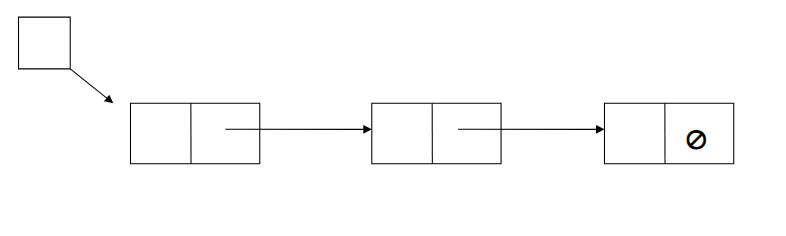
\includegraphics[width=0.5\textwidth]{rappresentazione_collegata_lista}
	\end{figure}
	Si puo' notare che si usa un riferimento al primo elemento della lista, detto \textit{riferimento iniziale} e un simbolo speciale $\emptyset$ come riferimento associato all'ultimo nodo, nel caso in cui la lista sia vuota, tale simbolo compare direttamente al riferimento iniziale. 
\end{document}